\chapter{Introduction}
\label{chap:intro}
The Artificial Intelligence (AI) spectrum is vast and complex. The diversity amongst models, as well as its constant evolution, makes it difficult to accurately categorize the existing paradigms. Two complimentary categories can be identified \citep{lieberman_symbolic_nodate}: symbolic and subsymbolic. \textit{Symbolic} models use human-readable inputs, and their inference processes can be fully understood and explained by humans. On the contrary, \textit{subsymbolic} models are based on arithmetical representation and statistical reasoning, thus offering enhanced reasoning capacity at the cost of being opaque to humans. This general categorization is narrowed in \cite{hopgood_2009_knowledge-based}, where the AI spectrum is divided into knowledge-based systems (symbolic) and computationally intelligent systems (subsymbolic). The latter are starting to include deep learning since its recent breakthrough.

Even though symbolic and subsymbolic models are generally treated independently, both types present complimentary properties. Therefore, if properly combined, the integration of both paradigms can lead to new, enhanced approaches that combine their benefits. Neurosymbolic AI explores this idea, comprising a set of approaches or methods for neurosymbolic system formulation, depicting the key features that should be exhibited \citep{mcgarry_hybrid_1999}, the criteria on which they should be rooted \citep{mira_neurosymbolic_2004}, or follow \citep{besold_neural-symbolic_2017}. Neurosymbolic approaches can be also approached according to the coupling degree between the models involved \citep{medsker2020models,hilario_overview_nodate}.

Neurosymbolic approaches can be broken down into two main categories from a general integration perspective: introduction (or insertion)\footnote{The terms ``introduction'' and ``insertion'' are used as synonyms throughout this thesis.}, and extraction. Insertion approaches integrate the different models under a unified framework, while one of the models is mined (or used to mine) from the other in extraction approaches.

Regarding the insertion of deep learning (DL) into knowledge-based systems (KBS), the most prominent integration comprises neural networks and rules \citep{daniele_knowledge_2019,hatzilygeroudis_integrated_2010}. More recently, with the resurfacing of knowledge graphs, this type of integration is starting to gain relevance. Knowledge graph completion \citep{nickel_review_ml_kg_2016,wang_kge_survey_2017,rossi_knowledge_2021} is one of the primary tasks regarding knowledge graphs, where the goal is to find new potential elements from the information modelled in the graph. This task is usually performed by knowledge graph embedding models \citep{transe,distmult,crosse}, which are frequently based on deep learning. 

Most of the extraction approaches are encompassed in the area of explainable artificial intelligence, whose goal is to mine insights on the inference process of deep learning models. According to \cite{burkart_survey_2021}, AI models should be explainable and exhibit features such as \textit{trust, causality, transferability,} or \textit{fair and ethical decision making}. These features are not intrinsic to deep learning models, which motivates extensive research on this direction.

The neurosymbolic design methods existing in the literature provide a grounding foundation on \textit{why} the integration is benefitial, and the features that the final system should exhibit. However, no insights are provided on \textit{how} to design these systems. Hence, there is a remarkable absence of guidelines on the design of neurosymbolic models. Besides the existing reasons for integration, the precise limitations of the symbolic and subsymbolic paradigms that motivate the need for a neurosymbolic model should be clearly outlined. Contextual and practical aspects should be also considered, such as the task to be performed, the available resources, or the data types required.

In addition to the theoretical aspects of neurosymbolic system design, there exists a lack of instantiation examples. Subsequently, a considerable number of potentially successful pairings are dismissed. Showcasing the versatility, adaptability, and benefits of neurosymbolic integration across different open research challenges will further motivate its usage, while providing a baseline for their future reuse. 

The research conducted in this thesis stems from the lack of neurosymbolic design guidelines and the limited number of instantation examples. The main goal of this thesis is to propose a general design method for neurosymbolic integration of KBS and DL models, comprising theoretical and practical aspects, that can be instantiated on a wide variety of model pairings and case scenarios. First, the limitations existing in previous neurosymbolic designs are addressed. In addition to the lack of design guidelines, previous works do not provide a specific insight on the limitations that motivate the need for a neurosymbolic model. A general design method is formulated for this purpose, comprising four different dimensions: \textit{limitations, considerations, restrictions}, and \textit{benefits}. Therefore, it integrates and extends the previously existing designs, yielding a full design frame for the characterization of any possible instance. According to the two main types of integration (insertion and extraction), four potential interactions between KBS and DL models can be established: two insertion interactions and two extraction interactions. However, the extraction of DL models from KBS is not feasible since subsymbolic models cannot be mined from their symbolic counterparts. Therefore, this thesis covers the following three interactions: KBS insertion into DL models, DL insertion into KBS, and KBS extraction from DL models. A specific design method for each of these interactions is formulated, referred to as interaction design methods. They provide a set of parameters for each of the four dimensions, addressing the context and particular features of each interaction. 

\begin{figure}
    \centering
    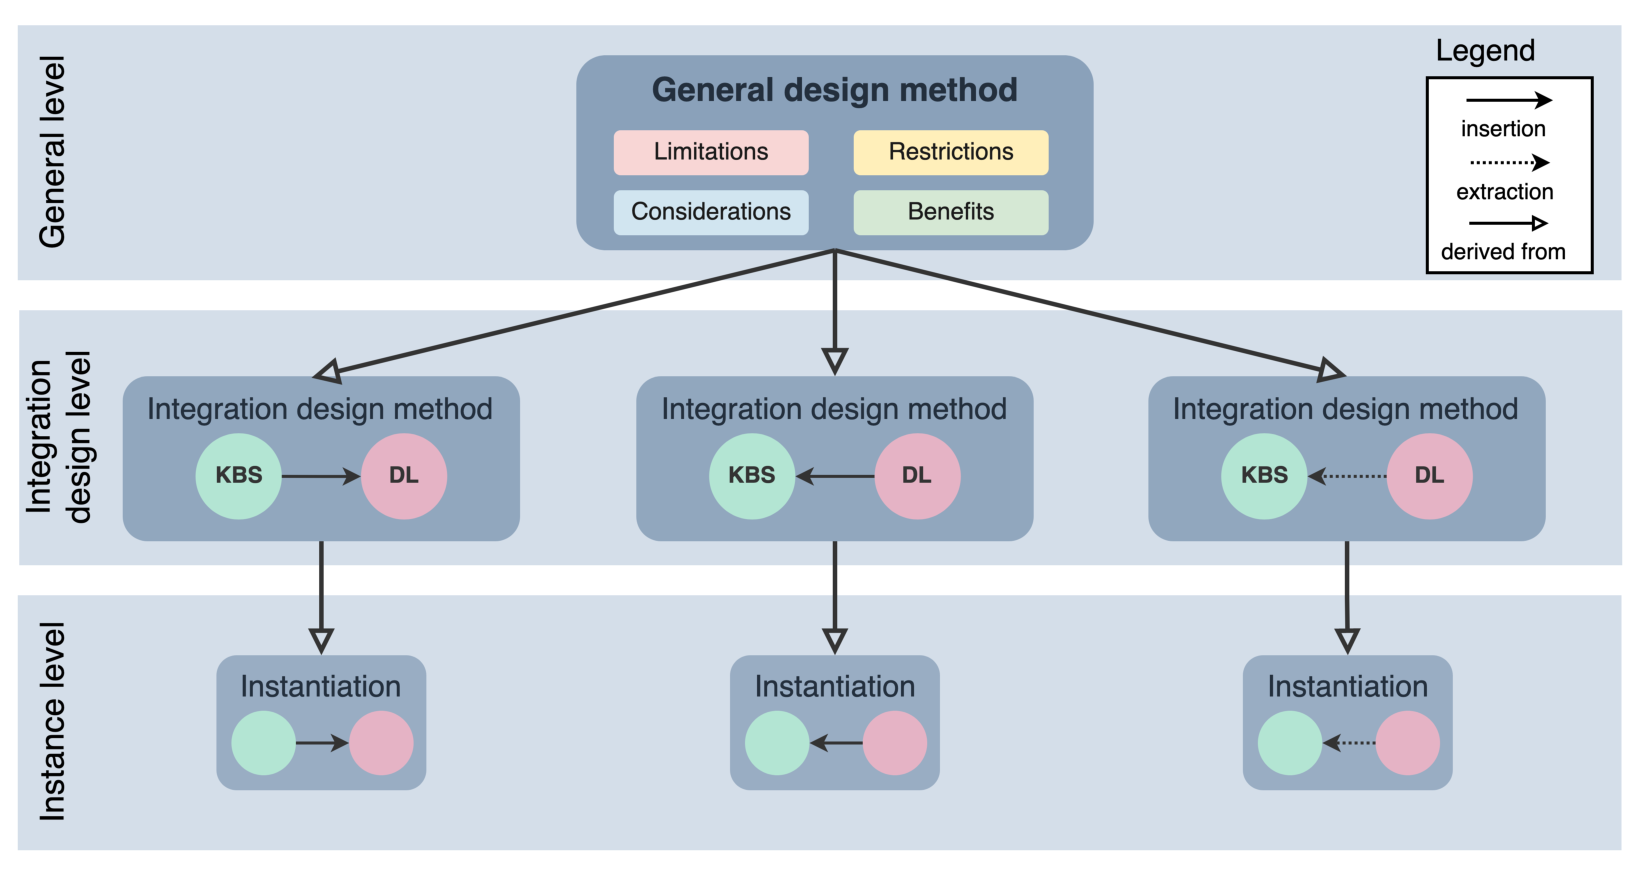
\includegraphics[width=\linewidth]{1_introduction/figures/hierarchy_method.eps}
    \caption{Hierarchical organization of the design method presented in this thesis.}
    \label{fig:hierarchy_design}
\end{figure}

Another important limitation is the staticity of the roles of symbolic and subsymbolic models in neurosymbolic integration. Symbolic paradigms are mostly related to representation tasks, disregarding their application as reasoning models. On the contrary, subsymbolic models are solely used for reasoning. Rule-based systems often portray a symbolic role, with neural networks being the most frequent reasoning paradigm. Therefore, a vast number of potential model interactions are dismissed. Instantiations of each of the three integration designs are presented to illustrate the versatility and usability of the proposed general design method. These instances showcase a variety of model pairings across different scenarios. Moreover, these instances address existing open research challenges on their specific application domains, subsequently contributing to their resolution. Figure \ref{fig:hierarchy_design} presents an overview on the organization of the different design levels covered in this thesis. 

In KBS insertion into DL models, a semantic-based initialization for knowledge graph completion is proposed, introducing ontologies into DL-based models. This integration not only improves the performance of the DL model, but accelerates its convergence while reducing the required data. A case-based reasoning model comprising several DL modules for medical document generation is presented in the second interaction (DL insertion into KBS). This framework combines the benefits of case-based reasoning with deep learning models, thus being user-centered and interpretable while providing results that can not be achieved without the inclusion of DL. In the third and final interaction, KBS extraction from DL, two different scenarios are presented, each tackling the problem of explainable AI from a different perspective. In the first scenario, a multi-agent system is devised to extract behavioral patterns from an opaque hyperpersonalization system, giving some insights on the associative patterns established by the system for content targeting. The second scenario continues the work initiated in the first interaction, presenting a framework capable of extracting explanations and insights from DL-based models for knowledge graph completion. 
%%Contexto
%%Motivacion
%%Objetivo general (1p)

\section{Thesis Structure}
The content presented in this thesis is distributed across seven chapters. Chapters four, five, and six follow the same internal structure. The thesis is organized as follows:
\begin{itemize}
    \item \textit{\textbf{Chapter \ref{chap:soa}} (State-of-the-art)} presents the existing work that supports and motivates the research in this thesis. First, an overview of the artificial intelligence spectrum is provided, presenting the different existing categorizations and their comprising models. An overview on neurosymbolic integration is then presented, focusing on three main aspects: motivation, design methods, and categorization. Existing neurosymbolic approaches are then presented and categorized into the two types of interactions contemplated in this thesis: insertion and extraction.
    
    \item \textit{\textbf{Chapter \ref{chap:methodology}} (Problem Statement, Goals, and Research Methodology)} introduces the research problem attained in this thesis, as well as presenting an overview on the research hypotheses, objectives, assumptions, contributions, and restrictions formulated for its resolution. The followed research methodology is also presented.
    
    \item \textit{\textbf{Chapter \ref{chap:kbsintegrationdl}} (Knowledge-Based System Introduction into Deep Learning Models)} explores the first of the covered integrations: the insertion of knowledge-based systems into deep learning models. The design method for this integration is described and instantiated in the context of knowledge graph completion.
    
    \item \textit{\textbf{Chapter \ref{chap:dlintegrationkbs}} (Deep Learning Introduction into Knowledge-Based Systems)} presents the second integration: deep learning introduction into knowledge-based systems. The design method for its integration is described and instantiated for the problem of medical document generation.
    
    \item \textit{\textbf{Chapter \ref{chap:kbsextractiondl}} (Knowledge-Based System Extraction from Deep Learning Models)} outlines the third integration: knowledge-based system extraction from deep learning models. The design method for this integration is presented and instantiated on two different application scenarios: behavioral pattern extraction from black-box hyperpersonalization policies, and insight and explanation extraction from knowledge graph embedding predictions.
    
    \item \textit{\textbf{Chapter \ref{chap:conc}} (Conclusions and Future Work)} draws the conclusions of the thesis, as well as future research lines. The research results generated during the thesis are also presented in this chapter.
\end{itemize}
